%%%%%%%%%%%%%%
%% Run LaTeX on this file several times to get Table of Contents,
%% cross-references, and citations.

%% If you have font problems, you may edit the w-bookps.sty file
%% to customize the font names to match those on your system.

%% w-bksamp.tex. Current Version: Feb 16, 2012
%%%%%%%%%%%%%%%%%%%%%%%%%%%%%%%%%%%%%%%%%%%%%%%%%%%%%%%%%%%%%%%%
%
%  Sample file for
%  Wiley Book Style, Design No.: SD 001B, 7x10
%  Wiley Book Style, Design No.: SD 004B, 6x9
%
%
%  Prepared by Amy Hendrickson, TeXnology Inc.
%  http://www.texnology.com
%%%%%%%%%%%%%%%%%%%%%%%%%%%%%%%%%%%%%%%%%%%%%%%%%%%%%%%%%%%%%%%%

%%%%%%%%%%%%%
% 7x10
%\documentclass{wileySev}

% 6x9
\documentclass{wileySix}

\usepackage{graphicx}
\usepackage{listings}
\usepackage{float}
\usepackage[urlcolor=blue, colorlinks=true]{hyperref}
\usepackage{textcomp}
\usepackage{color}
 
\definecolor{codegreen}{rgb}{0,0.6,0}
\definecolor{codegray}{rgb}{0.5,0.5,0.5}
\definecolor{codepurple}{rgb}{0.58,0,0.82}
\definecolor{backcolour}{rgb}{0.95,0.95,0.92}
 
\lstdefinestyle{mystyle}{
    backgroundcolor=\color{backcolour},   
    commentstyle=\color{codegreen},
    keywordstyle=\color{magenta},
    numberstyle=\tiny\color{codegray},
    stringstyle=\color{codepurple},
    basicstyle=\footnotesize,
    breakatwhitespace=false,         
    breaklines=true,                 
    captionpos=b,                    
    keepspaces=true,                 
    numbers=left,                    
    numbersep=5pt,                  
    showspaces=false,                
    showstringspaces=false,
    showtabs=false,                  
    tabsize=2,
    language=sh
}
 
\lstset{style=mystyle}

%%%%%%%
%% for times math: However, this package disables bold math (!)
%% \mathbf{x} will still work, but you will not have bold math
%% in section heads or chapter titles. If you don't use math
%% in those environments, mathptmx might be a good choice.

% \usepackage{mathptmx}

% For PostScript text
%\usepackage{w-bookps}

%%%%%%%%%%%%%%%%%%%%%%%%%%%%%%%%%%%%%%%%%%%%%%%%%%%%%%%%%%%%%%%%
%% Other packages you might want to use:

% for chapter bibliography made with BibTeX
% \usepackage{chapterbib}

% for multiple indices
% \usepackage{multind}

% for answers to problems
% \usepackage{answers}

%%%%%%%%%%%%%%%%%%%%%%%%%%%%%%
%% Change options here if you want:
%%
%% How many levels of section head would you like numbered?
%% 0= no section numbers, 1= section, 2= subsection, 3= subsubsection
%%==>>
\setcounter{secnumdepth}{3}

%% How many levels of section head would you like to appear in the
%% Table of Contents?
%% 0= chapter titles, 1= section titles, 2= subsection titles, 
%% 3= subsubsection titles.
%%==>>
\setcounter{tocdepth}{2}

%% Cropmarks? good for final page makeup
%% \docropmarks

%%%%%%%%%%%%%%%%%%%%%%%%%%%%%%
%
% DRAFT
%
% Uncomment to get double spacing between lines, current date and time
% printed at bottom of page.
% \draft
% (If you want to keep tables from becoming double spaced also uncomment
% this):
% \renewcommand{\arraystretch}{0.6}
%%%%%%%%%%%%%%%%%%%%%%%%%%%%%%

%%%%%%% Demo of section head containing sample macro:
%% To get a macro to expand correctly in a section head, with upper and
%% lower case math, put the definition and set the box 
%% before \begin{document}, so that when it appears in the 
%% table of contents it will also work:

\newcommand{\VT}[1]{\ensuremath{{V_{T#1}}}}

%% use a box to expand the macro before we put it into the section head:

\newbox\sectsavebox
\setbox\sectsavebox=\hbox{\boldmath\VT{xyz}}

%%%%%%%%%%%%%%%%% End Demo


\begin{document}


\booktitle{Cerdas Menguasai Git}
\subtitle{Dalam 24 Jam}

\authors{Rolly M. Awangga\\
\affil{Informatics Research Center}
%Floyd J. Fowler, Jr.\\
%\affil{University of New Mexico}
}

\offprintinfo{Cerdas Menguasai Git, First Edition}{Rolly M. Awangga}

%% Can use \\ if title, and edition are too wide, ie,
%% \offprintinfo{Survey Methodology,\\ Second Edition}{Robert M. Groves}

%%%%%%%%%%%%%%%%%%%%%%%%%%%%%%
%% 
\halftitlepage

\titlepage


\begin{copyrightpage}{2019}
\input{info/copyrightpage}
\end{copyrightpage}

\dedication{`Jika Kamu tidak dapat menahan lelahnya belajar, 
Maka kamu harus sanggup menahan perihnya Kebodohan.'
~Imam Syafi'i~}

\begin{contributors}
\input{info/contributors}
\end{contributors}

\contentsinbrief
\tableofcontents
\listoffigures
\listoftables
\lstlistoflistings


\begin{foreword}
\input{info/foreword}
\end{foreword}

\begin{preface}
\input{info/preface}
\end{preface}


\begin{acknowledgments}
\input{info/acknowledgments}
\end{acknowledgments}

\begin{acronyms}
\input{info/acronyms}
\end{acronyms}

\begin{glossary}
\input{info/glossary}
\end{glossary}

\begin{symbols}
\input{info/symbols}
\end{symbols}

\begin{introduction}
\input{info/introduction}
\end{introduction}

%%%%%%%%%%%%%%%%%%Isi Buku_

\chapter{Chapter 1}
\input{chapters/chapter1/1174006}
\section{ Arrizal Furqona Gifary / 1174070}
\subsection{Teori}

\begin{enumerate}

\item Jelaskan kenapa file suara harus dilakukan MFCC dilengkapi dengan ilustrasi atau gambar.\par
digunakan untuk mengidentifikasi jenis suara misalkan jenis suara gendre lagu jes pop metal dan klasikal atau suara ultra sonic.
\begin{figure}[ht]
\centering

\includegraphics[scale=0.5]{figures/1174070/6/1,1.PNG}
\caption{Ilustrasi gambar metode MFCC}
\label{contoh}
\end{figure}


\item Jelaskan konsep dasar neural network. dilengkapo dengan ilustrasi gambar. \par
konsep neural network dilaka ada inputan pasti ada outputan sesuai dengan kategori inputan dan fungsi di dalamnya.
\begin{figure}[ht]
\centering
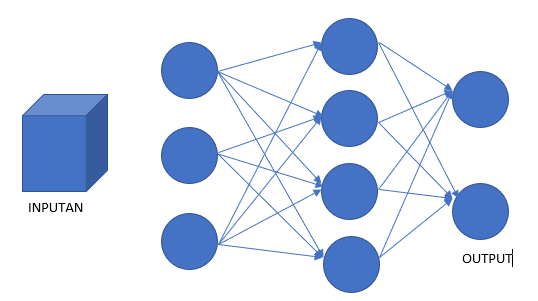
\includegraphics[scale=0.5]{figures/1174070/6/1,2.PNG}
\caption{Ilustrasi Konsep dasar neural network}
\label{contoh}
\end{figure}


\item Jelaskan konsep pembobotan  dalam neural network. dilengkapidengan ilustrasi gambar. \par
pembobotan dalam neural network yaitu digunakan untuk membedakan objek inputan atau variabel inputan untuk AI misalkan apel dan jeruk digunakan untuk variabel inputan maka dibuat pembobotan anatara kedua benda tersebut untuk menentukan output yang pasti dari inputan yang dilakukan.
\begin{figure}[ht]
\centering
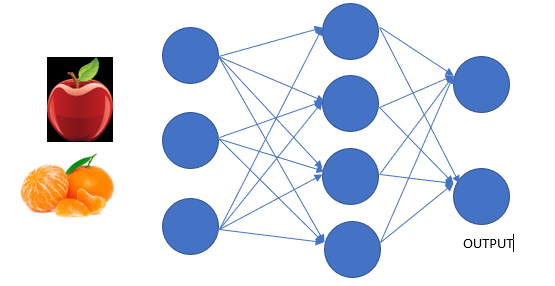
\includegraphics[scale=0.5]{figures/1174070/6/1,3.PNG}
\caption{Ilustrasi Konsep pembobotan pada neural network}
\label{contoh}
\end{figure}

\item Jelaskan konsep aktifitas dalam neural network. dilengkapi dengan ilustrasi gambar.\par
cara aktifitas dalam neural network dilakukan terhadap input pada neural network inputan tersebut dimasukan kepada fungsi pada mesin misalkan fungsi tanh(x) sehingga di hasilkanlah output yang sesuai dengan fungsi tersebut.
\begin{figure}[ht]
\centering
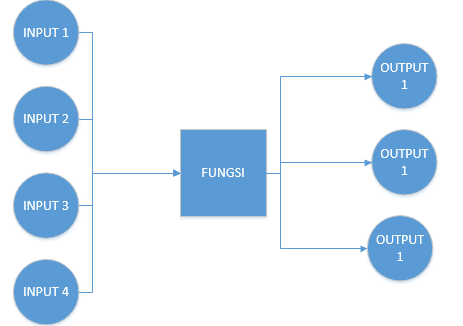
\includegraphics[scale=0.5]{figures/1174070/6/1,4.PNG}
\caption{Gambar yang dibaca hasil plotnya}
\label{contoh}
\end{figure}

\item Jelaskan cara membaca hasil plot dari MFCC dilengkapi dengan ilustrasi gambar. \par
cara membaca hasil ploting dari MFCC yaitu tentukan terlebih dahulu batas minimal Hz dari gelombang suara dan batas maksimal dari suara tersebut. kemudian warna yang paling pekat merupakan hasil dari pengolahan data tersebut misalkan muncul warna orange pekat di bagian bawah dan orange muda di bagian atas yang berarti suara tersebut kuat bagian basnya dan biasanya juga antara warna yang pekat tersebut ada jarak.
\begin{figure}[ht]
\centering
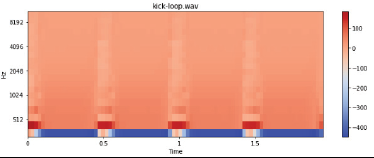
\includegraphics[scale=0.5]{figures/1174070/6/1,5.PNG}
\caption{Ilustrasi Cara Membaca Hasil Plot}
\label{contoh}
\end{figure}

\item Jelaskan apa itu one-hot encoding, dilengkapi dengan ilustrasi kode atau gambar.\par
one-hot encoding merupakan pemberian nilai pada suatu variabel jika nilai itu iya maka nilainya satu dan jika tidak maka nilainya nol.
\begin{figure}[ht]
\centering
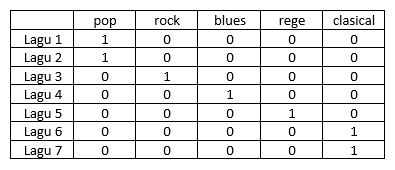
\includegraphics[scale=0.5]{figures/1174070/6/1,6.PNG}
\caption{Ilustrasi Konsep one-hot encoding}
\label{contoh}
\end{figure}

\item Jelaskan apa dari np.unique dan to\_categorical dalam kode program, dilengkapi dengan ilustrasi atau gambar.\par
digunakan untuk membuat array sedangkan  to\_categorical digunakan untuk membuat matrix baui itu 64 bit atau 32 bit.
\begin{figure}[ht]
\centering
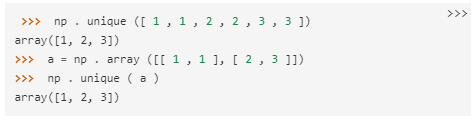
\includegraphics[scale=0.5]{figures/1174070/6/1,7,1.PNG}
\caption{Ilustrasi np.unique}
\label{contoh}
\end{figure}

\begin{figure}[ht]
\centering
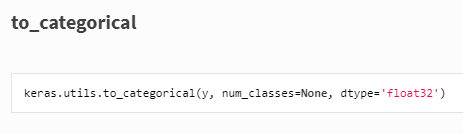
\includegraphics[scale=0.5]{figures/1174070/6/1,7,2.PNG}
\caption{Ilustrasi to\_categorical}
\label{contoh}
\end{figure}


\item Jelaskan apa fungsi dari Sequential dalam kode program, dilengkapi dengan ilustrasi atau gambar. \par
sequential adalah prosesperbandingan setiap elemen satu persatu mulai dari dari objek pertama hingga yang di tuju atau jika mencari angka 100 maka sequential akan membagi bagian misalnya dari satu sampai 20 dan seterusnya sampai mendapat nilai seratus.
\begin{figure}[ht]
\centering
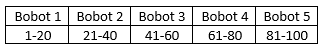
\includegraphics[scale=0.5]{figures/1174070/6/1,8.PNG}
\caption{Ilustrasi Konsep pembobotan pada neural network}
\label{contoh}
\end{figure}

\end{enumerate}

\subsection{Praktikum}
\begin{enumerate}
\item Jelaskan isi dari data GTZAN Genre Collection dan data dari freesound. Buat kode program program untuk meload data tersebut untuk digunakan pada MFCC. Jelaskan arti dari perbaris kode yang dibuat (harus beda dengan teman satukelas).\par
\subitem Isi data data merupakan datasets lagu atau suara yang tersiri dari 10 gendre yang di simpan kedalam 10 folder yaitu folder blues, classical, country, disco, hiphop, jazz, metal, pop, reggae, dan rock ke sepuluh folder tersebut masing-masing  berisi 100 data suara sedangkan data freesound merupakan contoh data suara yang akan di gunakan untuk menguji hasil pengolahan data tersebut dengan menggunakan metode mfcc. apakah suara dari freesound termasuk kategori jazz pop atau sebagainya ?.

\lstinputlisting{src/1174070/6/2,1.py}

\subitem dapat dilihat pada kode diatas pada baris kesatu dilakukan import librosa tang digunakan untuk fungsi mfcc pada suara.
pada baris kedua dilakukan import librosa featuse dan pada baris ke tiga dilakukan librosa display selanjutnya pada baris ke empat dilakukan import glob kemudian insert numpy untuk pengolahan data menjadi vektor setelah itu dilakukan import matplotlib untuk melakukan ploting setelah itu dilakukan import librari keras.\par

\subitem Selanjutnya yaitu membuat fungsi mfcc dengan nama display\_mfcc yang didalamnya terdapat variabel y yang berisi method librosa load kemudian variabel mfcc yang berisi method librosa featurea mfcc. Setelah itu membuat flot figure dengan ukuran 10 banding 4 kemudian di isi oleh data librosa display dengan variabel x nya yaitu waktu dan y yaitu mel atau Hz kemudian melakukan plot warna setelah itu melakukan plot judul dan terakhir flot di tampilkan. 

\item Jelaskan perbaris kode program dengan kata-kata dan di lengkapi ilustrasi gambar fungsi dari display\_mfcc().\par

\lstinputlisting{src/1174070/6/2,2.py}

\subitem pada baris ke dua program diatas digunakan untuk mendisplay tampilan glombang suara dari file 266093\_\_stereo-surgeon\_\_kick-loop-5.wav menggunakan metode mfcc dengan menggunakan fungsi display\_mfcc yang telah tadi di buat pada nomer dua begitu juga pada baris ke 4 6 8 sampai ke 22 secara teksis sama menggunakan fungsi display\_mfcc hanyasaja beda peyimpanan data yang akan di tampilkan atau di eksekusi. untuk contoh hasilnya dapat dilihat pada gambar \ref{c122} berikut:
\begin{figure}[ht]
\centering
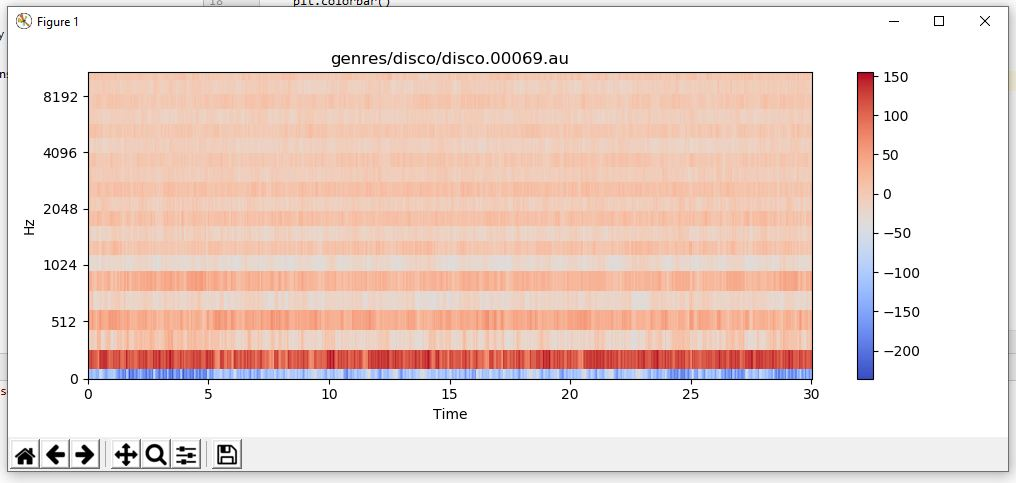
\includegraphics[scale=0.5]{figures/1174070/6/2,2.JPG}
\caption{Ilustrasi gambar fungsi dari display\_mfcc() }
\label{contoh}
\end{figure}

Gambar tersebut merupakan hasil dari mfcc dari salah satu gender lagu pop yang ada pada datasets yang 1000 atau terdapat dalam sepuluh folder tadi.

\item Jelaskan perbaris dengan kata-kata dan dilengkapi dengan ilustrasi gambar fungsi dari extract\_features\_song jelaskan kenapa data yangdiambil merupakan data 25.000 baris pertama ? 

\lstinputlisting{src/1174070/6/2,3.py}

\subitem pada baris ke tiga di definisikan nama extract\_features\_song yang nantinya akan di gunakan pada fungsi yang lainya kemudian dibuat variabel y dengan method librosa load setelah itu dibuat variabel baru mfcc dengan isi librosa features mfcc dengan isi variabel y tadi kemudian dibuat variabel mfcc dengan isian np.max dan variabel mfcc tadi terakhir di buat array dari data tersebut merupakan data 25000 data pertama. kenapa data 25000 pertama yang digunakan dikarenakan data tersebut digunakan sebagai data testing semakin besar data testing yang di gunakan maka semakin akurat hasil AI. tapi sebenarnya data tersebut relatif bisa lebih besar atau lebih kecil tergantung pada komputer masing masing.

\item Jelaskan Perbaris kode program dengan kata-kata dan di lengkapi ilustrasi gambar fungsi dari generate features and labels.

\lstinputlisting{src/1174070/6/2,4.py}

\subitem pada baris ke tiga merupakan pendefinisian nama fungsi yaitu generate features and labels kemudian membuat variabel baru dengan array kosing yaitu all\_features dan all\_labels kemudian mendefinisikan isian label untuk gendre dengan cara membuat variabel genres kemudian di isi dengan 10 gendre yang tadi setelah itu dilakukan fungsi if else dengan code for dan in setelah itu akan di buat encoding untuk data tiap tiap label contoh untuk blues 1000000000 dan untuk clasical 0100000000.

\item Jelaskan dengan kata dan praktek kenapa penggunaan fungsi generate features and labels sangat lama saat meload dataset gendre tunjukan keluarannya dari komputer sendiri dan artikan maksud dari luaran tersebut.\par

halnini menjadi lama dikarenakan mesin membaca satupersatu file yang ada pada folder dan dalam foldertersebut terdapat 100 file sehingga wajar menjadi lama ditambah lagi mengolah data yang tadinya suara menjadi bentuk vektor. berikut merupakan codenya.
\lstinputlisting{src/1174070/6/2,5.py}
\begin{figure}[ht]
\centering
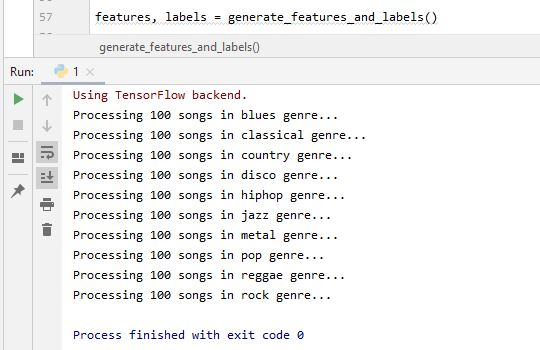
\includegraphics[scale=0.5]{figures/1174070/6/2,5.JPG}
\caption{Hasil dari fungsi generate features and labels}
\label{contoh}
\end{figure}


\item jelaskan kenapa harus dilakukan pemisahan data training dan data testing sebesar 80 persen praktekan dengan kode dan tunjukan keluarannya dari komputer sendiri dan artikan maksud dari luaran tersebut. 
untuk code nya adalah sebagai berikut  yang merupakan code untuk membagi data sebanyak 80 persen untuk data training maka data musik tadi yang total jumlahnya 1000 akan di bagi dua untuk data training sebanyak 800  dan 200 untuk data testing.
\lstinputlisting{src/1174070/6/2,6.py}


\item praktekan dan jelaskan masing masing parameter dari fungsi Sequential().  tunjukan keluarannya dari komputer sendiri dan artikan maksud dari luaran tersebut.\par
\subitem fungsi sequential digunakan untuk mengolah data inputan sesuai dengan fungsi yang ada pada fungsi sequential pada fungsi sequential kali ini menggunakan dua fungsi sequential mengkompile data dari 100 neuron atau dari 1 folder file dengan menggunakan fungsi relu dan softmax untuk menghasilkan outputan yang sesuai dengan keriteria.
\lstinputlisting{src/1174070/6/2,7.py}


\item praktekan dan jelaskan masing masing parameter dari fungsi compile().  tunjukan keluarannya dari komputer sendiri dan artikan maksud dari luaran tersebut. \par
\subitem yaitu fungsi kompile yang digunakan untuk mengetahui parameter yang digunakan dari data yang telah diolah untuk caranya dapat menggunakan codingan sebagai berikut, pada gambar tersebut memunculkan parameternya berapasaja dan total parameter yang digunakan.
\lstinputlisting{src/1174070/6/2,8.py}
\begin{figure}[ht]
\centering
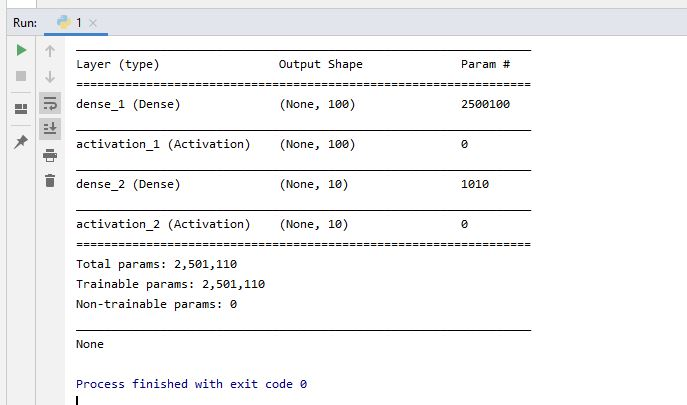
\includegraphics[scale=0.5]{figures/1174070/6/2,8.JPG}
\caption{Hasil fungsi compile}
\label{contoh}
\end{figure}

\item praktekan dan jelaskan masing masing parameter dari fungsi fit().  tunjukan keluarannya dari komputer sendiri dan artikan maksud dari luaran tersebut.\par
\subitem pada fungsi ini dilakukan pengolahan data dari 10 label tadi atau 10 file data sets tadi kemudian di hitung tingkat akurasi masing masing dan tingkat kegagalan atau loss data darisetiap file tersebut caranya dengan melakukan codingan berikut. pada gambar tersebut menunjukan 10 pengolahan data untuk menentukan nilai akurasi dan loss dari data tersebut dan selanjutnya dilakukan fingsi evaluasi.
\lstinputlisting{src/1174070/6/2,9.py}
\begin{figure}[ht]
\centering
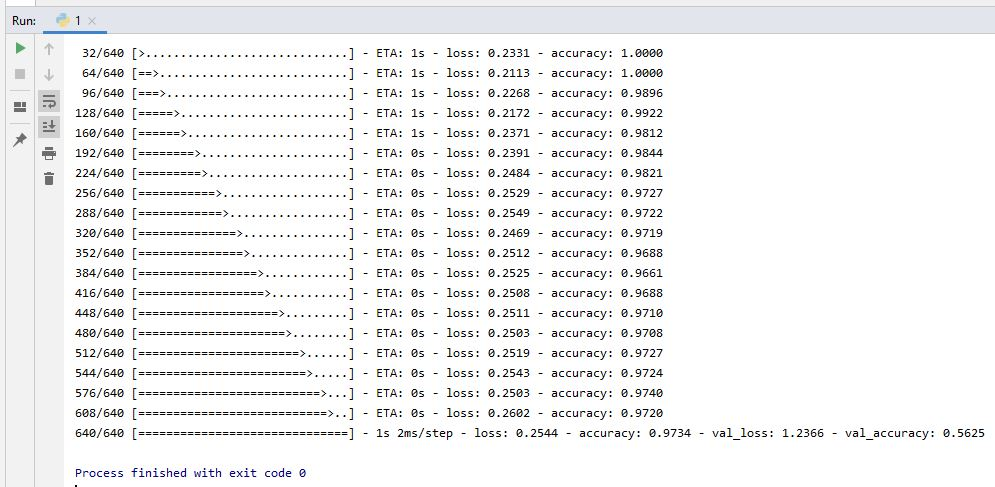
\includegraphics[scale=0.5]{figures/1174070/6/2,9.JPG}
\caption{Hasil fungsi fit}
\label{contoh}
\end{figure}

\item praktekan dan jelaskan masing masing parameter dari fungsi evaluate().  tunjukan keluarannya dari komputer sendiri dan artikan maksud dari luaran tersebut.\par
\subitem pada fungsi ini dilakukan evaluasi terhadap datayang telah di runing sebelummnya untuk lebih jelasnya dapat di lihat codingan tersebut  pada codingan tersebut dilakukan evaluasi pada tingkat kegagalan dan akurasi kebenaran maka hasilnya munculkan hasil evaluasi dari 10 proses dari setiap gendre yaitu akurasi sebesar 51 persen dan loss data sebesar 1.4105 data.
\lstinputlisting{src/1174070/6/2,10.py}
\begin{figure}[ht]
\centering
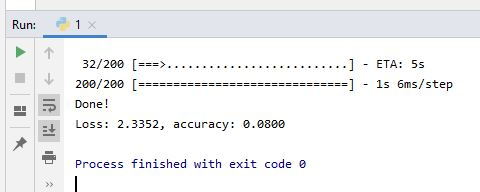
\includegraphics[scale=0.5]{figures/1174070/6/2,10.JPG}
\caption{Hasil fungsi evaluasi}
\label{contoh}
\end{figure}

\item praktekan dan jelaskan masing masing parameter dari fungsi predic  tunjukan keluarannya dari komputer sendiri dan artikan maksud dari luaran tersebut. \par 
\subitem fungsi predic merupakan fungsi untuk membandingkan tingkat akurasi pada setiap label yang sepuluh tadi maka data akan di sandingkan ke masing masing tingkat akurasinya, yang akurasinya paling tinggi maka itulah jawaban untuk setiap inputan yang dilakukan. 
\lstinputlisting{src/1174070/6/2,11.py}
\begin{figure}[ht]
\centering
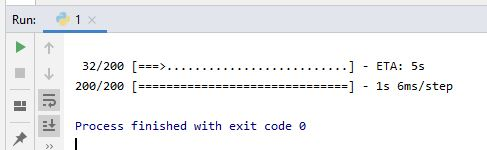
\includegraphics[scale=0.5]{figures/1174070/6/2,11.JPG}
\caption{Hasil fungsi prediksi}
\label{contoh}
\end{figure}

Alhamduluillah
\end{enumerate}


\section{Fanny Shafira Damayanti (1174069)}
\subsection{Teori}
\begin{enumerate}
\item Definisi Kecerdasan buatan\\ 
Kecerdasan buatan atau Artificial intelligence merupakan kecerdasan yang ditambahkkan kedalam suatu system yang diatur secara ilmiah. Kecerdasan buatan dibuat untuk menggantikan pekerjaan yang dilakukan oleh manusia menjadi dikerjakan oleh sistem.

\item Sejarah Kecerdasan Buatan
\begin{itemize}
\item Abad 17, Rene Descartes berkata bahwa tubuh hewan adalah sekumpulan mesin yang rumit.
\item 1642, Blaise Pascal menciptakan mesin penghitung digital mekanis pertama.
\item Abad 19, Charles Babbage dan Ada Lovelace bekerja di program penghitung mekanis.
\item 1950, John McCarthy membuat istilah “Kecerdasan Buatan”.
\item 1960-1970, Joel Moses membuat program yang pertama kali sukses dalam bidang matematika.
\item 1980, jaringan saraf digunakan secara meluas dengan algoritme perambatan balik.
\item 2004, DARPA membuat kendaraan yang bisa dijalankan sendiri tanpa manusia.
\end{itemize}

\item Perkembangan kecerdasan buatan
\begin{itemize}
\item Masa persiapan (1943-1946)
Warren McCulloch dan Walter Pitt mengemukakan tiga hal : pengetahuan fisiologi dasar dan fungsi sel syaraf dalam otak, analisa formal tentang logika proposisi, dan teori komputasi Turing.

Pada tahun 1950, Nobert Wiener membuat penelitian mengenai prinsip-prinsip teori feedback.

Pada tahun 1956, John McCarthy meyakinkan Minsky, Claude Shannon dan Nathaniel Rochester untuk membantunya melakukan penelitian dalam bidan Otomata, Jaringan Syaraf dan pembelajaran intelijensia. 

\item Awal perkembangan (1952-1969)
Pada tahun 1958, McCarthy di MIT AI Lab Memo No.1 mendefinisikan bahasa pemrograman tingkat tinggi yaitu LISP,

Pada tahun 1959, Nathaniel Rochester dari IBM dan mahasiswa-mahasiswanya mengeluarkan program kecerdasan buatan yaitu Geometry Theorm Prover.

Pada tahun 1963, program yang dibuat James Slagle mampu menyelesaikan masalah integral tertutup untuk mata kuliah Kalkulus.
Pada tahun 1986, program analogi buatan Tom Evan menyelesaikan masalah analogi geometris yang ada pada tes IQ.

\item Perkembangan Kecerdasan Buatan Melambat (1969-1979)
Bruce Buchanan dan Joshua Lederberg yang membuat program untuk memecahkan masalah struktur molekul dari informasi yang didapatkan dari spectrometer massa.

\item AI Menjadi sebuah industri
Industrialisasi kecerdasan buatan diawali dengan ditemukannya sistem pakar yang dinamakan R1 yang mampu mengkonfigurasi system-sistem computer baru. 

\item Kembalinya Jaringan Syaraf Tiruan (1986-sekarang)
Pada tahun 1985-an setidaknya empat kelompok riset menemukan kembali algoritma belajar propagasi balik (Black-Propagation Learning). Algoritma ini berhasil diimplementasikan ke dalam bidang ilmu computer dan psikologi.
\end{itemize}

\item Definisi Supervised Learning\\
Supervised Learning merupakan cabang dari Artificial Intelligence. supervised learning adalah suatu ilmu yang mempelajari perancangan dan pengembangan algoritma.

\item Klasifikasi Supervised Learning
\begin{itemize}
\item Logistic regression.
\item K-nearest neighbors.
\item Support vector machine (SVM)
\item Naive Bayes.
\item Decision tree classification.
\item Random forest classification.
\end{itemize}

\item Regresi dan Unsupervised Learning\\
Regresi merupakan sebuah metode analisis statistic yang digunkan untuk mengetahui pengaruh antara dua variable atau lebih.

Untuk mempelajari Unsupervised learning kita tidak perlu data training untuk melakukan prediksi maupun klasifikasi.

\item Dataset\\
Dataset merupakan objek yang mempresentasikan data dan relasinya pada memori.

\item Training Set\\
Training Set merupakan bagian dari dataset untuk membuat prediksi atau menjalankan fungsi dari sebuah algoritma Machine Learning.

\item Testing Set\\
Testing set digunakan untuk mengukur apakah classifier berhasil melakukan klasifikasi dengan benar.

\end{enumerate}

\subsection{Instalasi}
\begin{enumerate}
	\item Instalasi Library scikit dari anaconda, mencoba kompilasi dan uji coba ambil contoh kode dan lihat variabel explorer
	\hfill\break
	\begin{figure}[H]
		\includegraphics[width=4cm]{figures/1174069/1/1.PNG}
		\centering
		\caption{Instalasi Package Scikit Learn}
	\end{figure}
	\begin{figure}[H]
		\includegraphics[width=4cm]{figures/1174069/1/2.png}
		\centering
		\caption{Isi Variabel Explorer}
	\end{figure}
	\item Mencoba Loading an example dataset, menjelaskan maksud dari tulisan tersebut dan mengartikan           		  per baris
	\hfill\break
	\lstinputlisting[firstline=7, lastline=11]{src/1174069/1/1174069.py}
	\item Mencoba Learning and predicting, menjelaskan maksud dari tulisan tersebut dan mengartikan per  			  baris
	\hfill\break
	\lstinputlisting[firstline=13, lastline=22]{src/1174069/1/1174069.py}
	\item  Mencoba Model persistence, menjelaskan maksud dari tulisan tersebut dan mengartikan per baris
	\hfill\break
	\lstinputlisting[firstline=25, lastline=34]{src/1174069/1/1174069.py}
	\item Mencoba Conventions, menjelaskan maksud dari tulisan tersebut dan mengartikan per baris
	\hfill\break
	\lstinputlisting[firstline=37, lastline=48]{src/1174069/1/1174069.py}
\end{enumerate}

\subsection{Penanganan Error}
\begin{enumerate}
	\item ScreenShoot Error
	\begin{figure}[H]
		\includegraphics[width=4cm]{figures/1174069/1/error/1.png}
		\centering
		\caption{Import Error}
	\end{figure}

	\item Tuliskan Kode Error dan Jenis Error
	\begin{itemize}
		\item Import Error
	\end{itemize}
	\item Cara Penangan Error
	\begin{itemize}
		\item Import Error
		\hfill\break
		Dengan Menginstall Library Yang Tidak Ditemukan
	\end{itemize}
\end{enumerate}

\subsection{Bukti Tidak Plagiat}
\begin{figure}[H]
	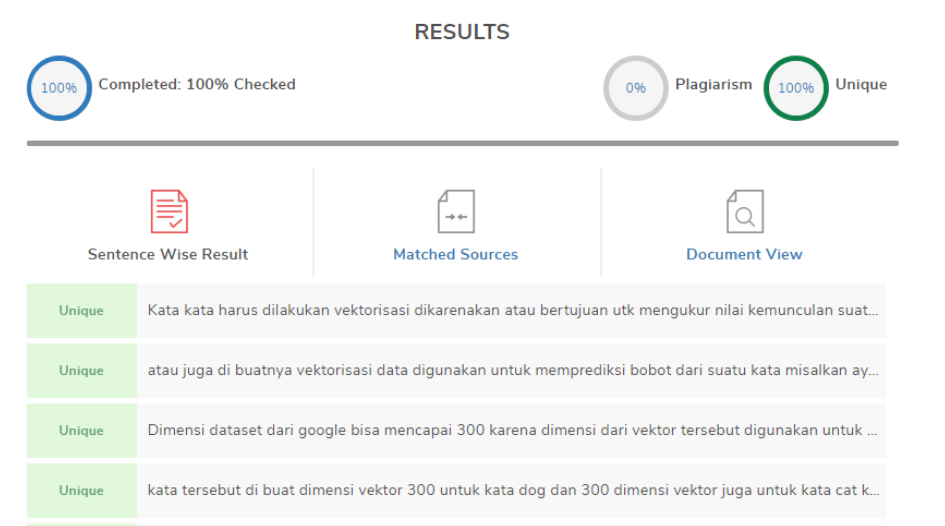
\includegraphics[width=4cm]{figures/1174069/1/plagiat/plagiat.PNG}
	\centering
	\caption{Bukti Tidak Melakukan Plagiat Chapter 1}
\end{figure}

\subsection{Link Youtube}
https://youtu.be/Ra4Lu-C8OQY

\section{Tia Nur Candida - 1174086}
\subsection{Teori}
\begin{enumerate}
\item Definisi Kecerdasan Buatan \\
Kecerdasan Buatan adalah suatu ilmu yang mempelajari bagaimana cara komputer melakukan sesuatu seperti yang dilakukan oleh manusia. Secara sederhana AI adalah teknik dan ilmu untuk membangun atau membuat suatu mesin menjadi cerdas, terutama pada program komputer. Kecerdasan yang dimaksud yaitu seperti yang dimiliki oleh manusia namun pada mesin akan dibuat cepat dan tepat atau akurat.

\item Sejarah Kecerdasan Buatan \\
Sejarah kecerdasan buatan dimulai pada zaman kuno. Benih kecerdasan buatan modern ditanamkan oleh filusuf klasik dengan berusaha menggambarkan proses berpikir manusia. Karya tersebut memuncak pada penemuan komputer digital yang di program pada tahun 1940 an, dimana terdapat sebuah mesin yang didasarkan pada esensi abstrak penalaran matematika. 
Istilah kecerdasan buatan pertama kali dikemukaan pada tahun 1956 di Konferensi Darthmouth yang kemudian sejak saat itu kecerdasan buatan terus berkembang.

\begin{itemize}
\item Masa Persiapan AI (1943-1956)\\
Pada tahun 1943, Warren McCulloch dan Walter Pitt mengemukakan tiga hal : pengetahuan fisiologi dasar dan fungsi sel syaraf dalam otak, analisa formal tentang logika proposisi, dan teori komputasi Turing. Mereka berhasil membuat suatu model sel syaraf tiruan dimana setiap sel syaraf digambarkan sebagai ‘on’ dan ‘off’. Mereka menunjukkan bahwa setiap fungsi dapat dihitung dengan suatu jaringan sel syaraf dan bahwa semua hubungan logis dapat diimplementasikan dengan struktur jaringan yang sederhana.
Pada tahun 1950, Nobert Wiener membuat penelitian mengenai prinsip-prinsip teori feedback. Contoh yang terkenal adalah thermostat. Penemuan ini juga merupakan awal dari perkembangan AI.

Pada tahun 1956, John McCarthy meyakinkan Minsky, Claude Shannon dan Nathaniel Rochester untuk membantunya melakukan penelitian dalam bidan Otomata, Jaringan Syaraf dan pembelajaran intelijensia. Mereka mengerjakan proyek ini selama 2 bulan di Dartsmouth. Hasilnya adalah program yang mampu berpikir non-numerik dan menyelesaikan masalah pemikiran, yang dinamakan Principia Mathematica. Hal ini menjadikan McCarthy disebut sebagai bapak kecerdasan buatan.


\item Awal perkembangan AI (1952-1969)\\
Kecerdasan buatan banyak mengalami kesuksesan pada tahun pertama. 
Pada tahun 1958, McCarthy di MIT AI Lab Memo No.1 mendefinisikan bahasa pemrograman tingkat tinggi yaiyu LISP, yang sekarang mendominasi pembuatan program-pogram kecerdasan buatan. Kemudian, McCarthy membuat program yang dinamakan Programs with Common Sense. Di dalam program tersebut, dibuat rancangan untuk menggunakan pengetahuan dalam mencari solusi.
Pada tahun 1959, Nathaniel Rochester dari IBM dan mahasiswa-mahasiswanya mengeluarkan program kecerdasan buatan yaitu Geometry Theorm Prover. Program ini dapat mengeluarkan suatu teorema menggunakan aksioma-aksioma yang ada.
Pada tahun 1963, program yang dibuat James Slagle mampu menyelesaikan masalah integral tertutup untuk mata kuliah Kalkulus.
Pada tahun 1986, program analogi buatan Tom Evan menyelesaikan masalah analogi geometris yang ada pada tes IQ.

\item Perkembangan kecerdasan buatan melambat (1966-1974)
Banyak masalah yang perlu di selesaikan oleh kecerdasan buatan dan baru sedikit program yang keluar menyebabkan melambat.

\item Kecerdasan buatan menjadi sebuah industri ( 1980 - 1988 )\\
Industrialisasi kecerdasan buatan diawali dengan ditemukannya sistem pakar yang dinamakan R1 yang mampu mengkonfigurasi system-sistem computer baru. Program tersebut mulai dioperasikan di Digital Equipment Corporation (DEC), McDermott, pada tahun 1982.
Pada tahun 1986, R1 telah berhasil menghemat US Dolar 40 juta per tahun.
Pada tahun 1988, kelompok kecerdasan buatan di DEC menjalankan 40 sistem pakar. Hampir semua perusahaan besar di USA mempunyai divisi AI. Sehingga perusahaan yang sejak tahun 1982 hanya menghasilkan beberapa juta US dolar per tahun meningkat menjadi 2 milyar US dolar per tahun pada tahun 1988.

\item Kembalinya Jaringan Syaraf Tiruan ( 1986 - Sekarang )\\
Meskipun bidang ilmu computer menolak jaringan syaraf tiruan setelah diterbitkannya buku “Perceptrons” karangan Minsky dan Papert, tetapi para ilmuwan masih mempelajari bidang ilmu tersebut dari sudut pandang yang lain yaitu fisika. Para ahli fisika seperti Hopfield (1982) menggunakan teknik-teknik mekanika statistika untuk menganalisa sifat-sifat pentimpanan dan optimasi pada jaringan syaraf. Para ahli psikologi, David Rumelhart dan Geoff Hinton, melanjutkan penelitian mengenai model jaringan syaraf tiruan pada memori.
Pada tahun 1985-an setidaknya empat kelompok riset menemukan kembali algoritma belajar propagasi balik (Black-Propagation Learning). Algoritma ini berhasil diimplementasikan ke dalam bidang ilmu computer dan psikologi.

\end{itemize}
\item Definisi Supervised Learning \\
Merupakan tipe Machine Learning dimana model ini menyediakan training data berlabel. Supervised learning merupakan suatu pembelajaran yang terawasi dimana jika output yang diharapkan telah diketahui sebelumnya.  Supervised Learning adalah tipe learning di mana kita mempunyai variable input dan variable output, dan menggunakan satu algoritma atau lebih untuk mempelajari fungsi pemetaan dari input ke output. Goal-nya adalah untuk memperkirakan fungsi pemetaannya, sehingga ketika kita mempunya input baru, kita dapat memprediksi output untuk input tersebut.

\item Klasifikasi
\begin{itemize}
\item Logistic regression
\item K-nearest neighbors
\item Support vector machine (SVM)
\item Naive Bayes
\item Decision tree classification
\item Random forest classification
\end{itemize}

\item Regresi \\
Regresi adalah suatu metode analisis statistik yang digunakan untuk melihat pengaruh antara dua atau lebih banyak variabel. Hubungan variabel tersebut bersifat fungsional yang diwujudkan dalam suatu model matematis.

\item Unsupervised Learning \\
Unsupervised Learning adalah tipe learning di mana kita hanya mempunyai data masukan (input data) tetapi tidak ada output variable yang berhubungan.\\
Goal dari unsupervised learning adalah untuk memodelkan struktur dasar atau distribusi dalam data dengan tujuan untuk mempelajari data lebih jauh lagi, dengan kata lain, adalah menyimpulkan fungsi yang mendeskripsikan atau menjelaskan data.

\item Dataset \\
Dataset adalah objek yang merepresentasikan data dan relasinya di memory. Strukturnya mirip dengan data di database. Dataset berisi koleksi dari datatable dan datarelation.
\item Training Set \\
Training set adalah bagian dataset yang kita latih untuk membuat prediksi atau menjalankan fungsi dari sebuah algoritma ML lainnya sesuai tujuannya masing-masing. Kita memberikan petunjuk melalui algoritma agar mesin yang kita latih bisa mencari korelasinya sendiri.
\item Test Set \\
Test set adalah bagian dataset yang kita tes untuk melihat keakuratannya, atau dengan kata lain melihat performanya.

\end{enumerate}
\subsection{Praktek}
\begin{enumerate}
	\item Instalasi Library scikit dari anaconda, mencoba kompilasi dan uji coba ambil contoh kode dan lihat variabel explorer
	\hfill\break
	\begin{figure}[H]
		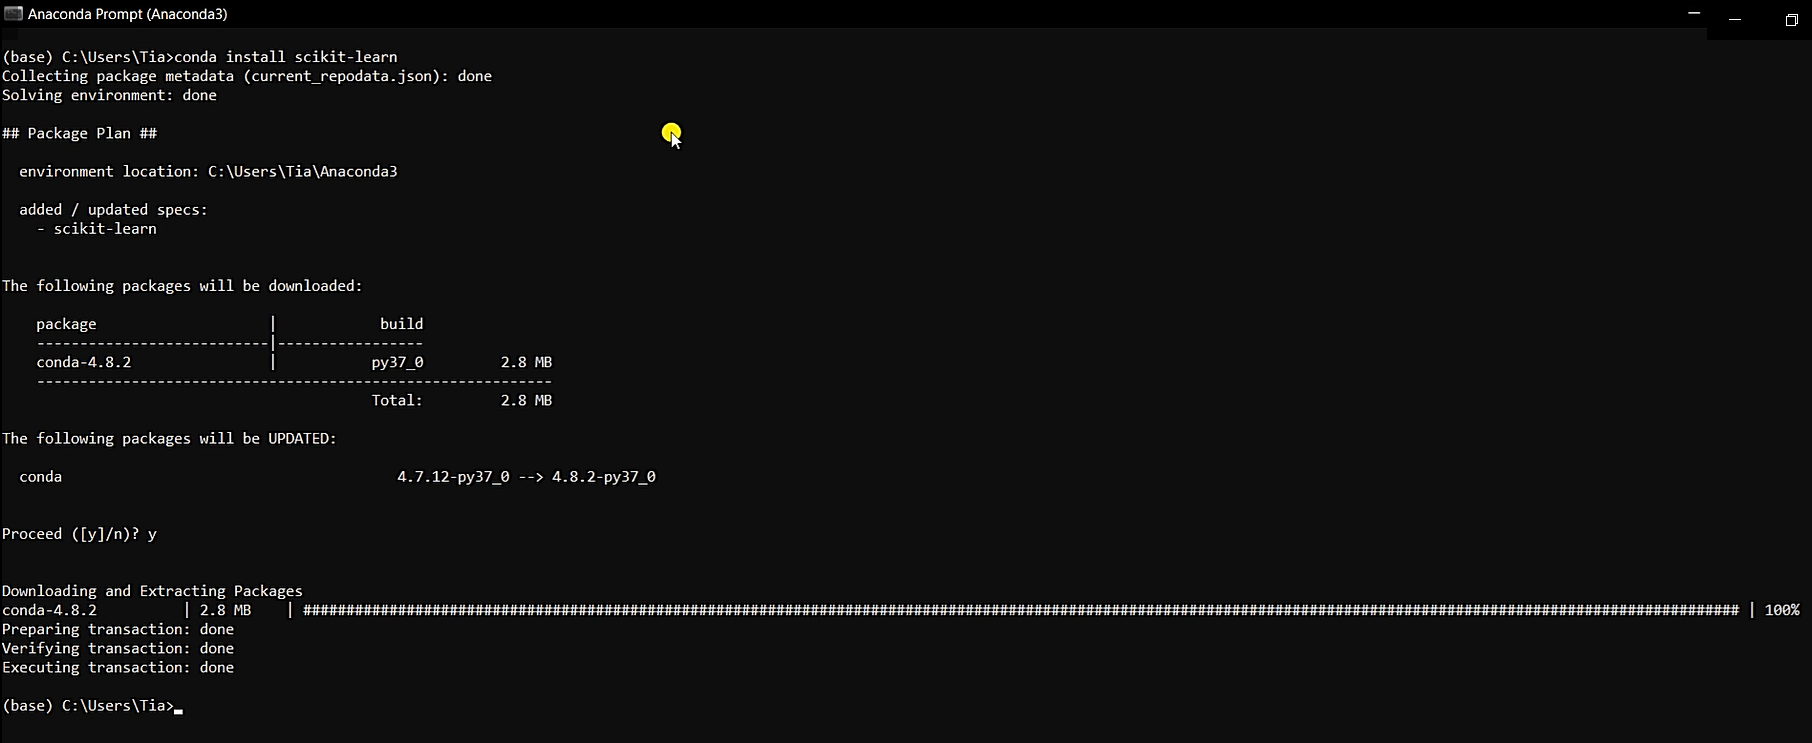
\includegraphics[width=4cm]{figures/1174086/1/installasi.PNG}
		\centering
		\caption{Instalasi Package Scikit Learn}
	\end{figure}
	\begin{figure}[H]
		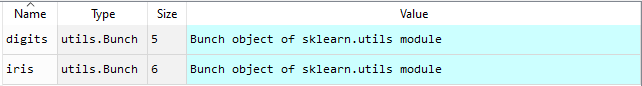
\includegraphics[width=4cm]{figures/1174086/1/variabel.png}
		\centering
		\caption{Isi Variabel Explorer}
	\end{figure}
	\item Mencoba loading an example dataset
	\hfill\break
	\lstinputlisting[firstline=7, lastline=11]{src/1174086/1/1174086.py}
	\item Mencoba Learning dan predicting
	\hfill\break
	\lstinputlisting[firstline=13, lastline=22]{src/1174086/1/1174086.py}
	\item Mencoba Model Persistence
	\hfill\break
	\lstinputlisting[firstline=25, lastline=34]{src/1174086/1/1174086.py}
	\item Mencoba Conventions
	\hfill\break
	\lstinputlisting[firstline=37, lastline=48]{src/1174086/1/1174086.py}
\end{enumerate}

\subsection{Bukti Tidak Plagiat}
\begin{figure}[H]
	\includegraphics[width=4cm]{figures/1174086/bukti/1.png}
	\centering
	\caption{Bukti Tidak Melakukan Plagiat Chapter 1}
\end{figure}


\section{1174054 | Aulyardha Anindita}

\subsection{Teori}
\begin{enumerate}
\item Definisi, Sejarah dan Perkembangan Kecerdasan Buatan
\begin{itemize}
\item Definisi Kecerdasan Buatan\\
Kecerdasan buatan adalah suatu kecerdasan yang didalamnya berisi suatu system yang biasa diatur dalam sebuah konteks ilmiah. Kecerdasan  buatan juga bisa didefinisikan sebagai sebuah kecerdasan yang diciptakan dan dimasukkan kedalam suatu mesin computer agar dapat melakukan pekerjaan seperti yang dapat dilakukan oleh manusia. Ada beberapa macam bidang atau ilmu yang menggunakan kecerdasan buatan diantaranya adalah system pakar, permainan computer (game), logika fuzzy, jaringan saraf tiruan dan robotika.\\
Penelitian dalam AI mencakup pembuatan mesin dan suatu program computer untuk mengotomatisasikan tugas-tugas yang membutuhkan perilaku cerdas, seperti : pengendalian, perencanaan dan penjadwalan serta kemampuan untuk menjawab diagnose dan pertanyaan pelanggan serta pengenalan tulisan tangan. Suara dan wajah

\item Sejarah Kecerdasan Buatan
\begin{itemize}
\item Pada tahun 1940 dan 1950 Artificial Inteligence merupakan suatu inovasi baru dalam bidang ilmu pengetahuan dimana pada tahun ini computer modern sudah ada
\item Pada tahun 1950 awal, studi tentang “mesin berfikir” mempunyai berbegai nama seperti cybernetics, teori automata, dan pemrosesan informasi
\item Pada tahun 1956, para ilmuwan jenius seperti Alan Turing, Norbert, Wiener, Claude Shannon dan Warren McCullough bekerja secara independen di bidang cybernetics, matematika, algoritma dan teori jaringan. John McCarthy merupakan orang yang menciptakan istilah tersebut dan mendirikan laboratorium kecerdasan buatan di MIT dan Stanford
\item Pada tahun 1956, McCarthy mendirikan Konferensi Dartmouth di Hanover, New Hampshire. Dia merupakan peneliti terkemuka dalam teori kompleksitas, simulasi Bahasa, dan hubungan antara keacakan dan pemikiran kreatif, jaringan saraf diundang. Sehingga Konferensi Dartmouth 1956 dianggap sebagai kelahiran Kecerdasan Buatan.
\item Sejak saat itu, Kecerdasan Buatan telah hidup melalui decade kemuliaan dan cemohan yang dikenal dengan luas sebagai musim panas dan musim dingin Ai.
\end{itemize}

\item Perkembangan Kecerdasan Buatan\\
Saat ini, teknologi Artificial Intelligence sangat ramai diperbincangkan oleh masyarakat. Sudah banyak pekerjaan yang hilang karena adanya AI, seperti pekerjaan kasir, penjaga pintu tol, parkir, dan sebagainya. Hal ini terjadi karena AI lebih unggul dalam hal kinerja, fitur dan lain sebagainya. Walaupun masih ada beberapa aspek yang memang pekerja manusia masih unggul dibandingkan AI itu sendiri. \\
Berdasarkan survei yang dilakukan oleh Microsoft, hasilnya adalah 39 responden masih mempertimbangkan untuk menggunakan mobil tanpa pengemudi dan sebanyak 36 responden lainnya setuju mahwa robot atau AI dengan menggunakan software untuk beroperasi mampu meningkatan produktivitas. Dari survei tersebut, dapat ditarik kesimpulan bahwa pengguna AI harus lebih bijaksana dalam pengembangan dan penggunaan dari AI sehingga tidak memiliki efek samping terhadap profuktifitas kerja dan keseharian sebagai pengguna dalam kehidupan sehari-hari.

\end{itemize}

\item Definisi Supervised Learning, Klasifikasi, Regresi, Unsupervised Learning, Data Set, Training Set dan Testing Set
\begin{itemize}
\item Supervised Learning\\
Supervised learning adalah suatu tugas pengumpulan data yang berfungsi untum menyimpulkan fungsi dari data pelatihan yang berlabel. Didalam Supervised Learning, setiap contoh merupakan pasangan yang terdiri dari objek input dan nilai output yang diinginkan. Algoritma pembelajaran yang diawasi berupa menganalisis data pelatihan dan menghasilkan fungsi yang disimpulkan yang digunakan untuk memetakan contoh baru.\\
 	Supervised Learning adalah suatu pendekatan dimana sudah terdapat data yang dilatih selain itu juga sudah memiliki variable yang ditargetkan sehingga tujuan dari pendekatan tersebut adalah mengelompokkan suatu data ke data yang sudah ada. Supervised learning sendiri menyediakan algoritma pembelajaran dengan jumlah yang diketahui untuk mendukung penilaian dimasa depan. Supervised learning sebagian besar memiliki kaitan dengan AI dengan menggunakan model pembelajaran generatif. Data pelatihan untuk pembelajaran yang diawasi mencakup beberapa contoh dengan subjek input yang berpasangan dan output yang diinginkan.\\
 	Modul supervised learning mempunyai beberapa keunggulan dibandingkan pendekatan tanpa pengawasan, tapi mereka juga memiliki keterbatasan. System lebih cenderung membuat penilaian bahwa manusia dapat berhubungan, misalnya manusia mempunyai dasar untuk keputusan. Tapi, dalam kasus tersebut yang menggunakan metode berbasis pengambilan, supervised learning mengalami kseulitan dalam menangani suatu informasi baru. 

\item Klasifikasi\\
Klasifikasi merupakan pembagian menurut kelas-kelas. Menurut ilmu pengetahuan, klasifikasi adalah suatu proses pengelompokkan benda berdasarkan ciri-ciri persamaan dan perbedaan. Dalam pembelajaran mesin dan statistic, klasifikasi merupakan suatu pendekatan pembelajaran yang diawasi dimana program computer tersebut belajar dari input data yang diberkan kepadanya lalu menggunakan pembelajaran tersebut untuk mengklasifikasikan pengamatan baru. Kumpulan data tersebut mungkin hanya bersifat dua kelas atau mungkin juga multi-kelas.

\item Regresi\\
Regresi adalah suatu metode analisis statistik yang digunakan untuk melihat pengaruh antara dua atau lebih variable. Regresi sendiri membahas masalah ketika variable output yaitu nilai ril atau berkelanjutan seperti gaji atau berat. Banyak model yang dapat digunakan, yang paling sederhana adalah regresi linear.

\item Unsupervised Learning\\
Unsupervised learning berbeda dengan supervised learning, perbedaanya yaitu unsupervised learning tidak memiliki data pelatihan, sehingga data dapat dikelompokkan menjadi dua atau 3 begitupun seterusnya. Unsupervised learning adalah suatu pelatihan algoritma kecerdasan buatan (AI) menggunakan beberapa informasi yang tidak diklasifikasikan atau diberi label dan memungkinkan algoritma  untuk bertindak atas informasi tersebut. System AI disini dapat dikelompokkan berdasarkan informasi yang tidak disortir berdasarkan persamaan dan perbedaan meskipun tidak ada kategori yang disediakan. System AI disajikan dengan data yang tidak berlabel, tidak terkategorisasi dan algoritma system bekerja pada data tanpa pelatihan sebelumnya sehingga outputmya tergantung pada algoritma kode.

\item Data Set\\
Data set adalah suatu objek yang merepresentasikan data dan memiliki relasi yang ada di dalam memory. Struktur data set mirip dengan data yang ada didatabase, namun bedanya data set berisi koleksi dari data table dan data relation. Untuk mendapatkan data yang tepat, berarti mengumpulkan atau mengidentifikasi data yang berkorelasi dengan hasil yang ingin anda prediksi.

\item Training Set\\
Training set adalah salah satu set yang biasa digunakan oleh algoritma klasifikasi. Seperti decision tree, bayesian, neural network, dll. Mereka dapat digunakan untuk membentuk model classifier, dalam menjalankan pelatihan yang diatur melalui jaringan saraf yang mengajarkan pada net dengan cara menimbang berbagai fitur, menyesuaikan koefisien berdasarkan kemungkinan mereka meminimalkan kesalahan. Kofiesen tersebut juga dikenal sebagai parameter.

\item Testing Set\\
Testing set adalah salah satu set yang digunakan untuk mengukur sejauh mana classifier berhasil melakukan klasifikasi dengan benar. Hal ini berfungsi sebagai materai persetujuan tapi tak digunakan sampai akhir. Setelah melatih dan mengoptimalkan data, kita dapat melakukan pengujian sarat terhadap pengambilan sampel aca. Dan hasilnya harus memvalidasi bahwa jaring data tersebut secara akurat mengenali gambar atau mengenali setidaknya (x) dari jumlah tersebut.

\end{itemize}
\end{enumerate}

\subsection{Praktek}
\begin{enumerate}
\item Instalasi library scikit dari anaconda
\hfill\break
	\begin{figure}[H]
		\includegraphics[width=4cm]{figures/1174054/1/1.png}
		\centering
		\caption{Instalasi Package Scikit Learn}
	\end{figure}
	\begin{figure}[H]
		\includegraphics[width=4cm]{figures/1174054/1/2.png}
		\centering
		\caption{Isi Variabel Explorer}
	\end{figure}
\item Mencoba Loading an example dataset
\hfill\break
	\lstinputlisting[firstline=8, lastline=12]{src/1174054/1/1174054.py}
	
\item Mencoba Learning and predicting
\hfill\break
	\lstinputlisting[firstline=14, lastline=24]{src/1174054/1/1174054.py}
	
\item Mencoba Model persistence
\hfill\break
	\lstinputlisting[firstline=26, lastline=36]{src/1174054/1/1174054.py}
	
\item Mencoba Conventions
\hfill\break
	\lstinputlisting[firstline=38, lastline=50]{src/1174054/1/1174054.py}
\end{enumerate}

\subsection{Penanganan Error}
\begin{enumerate}
\item ScreenShoot Error
	\begin{figure}[H]
		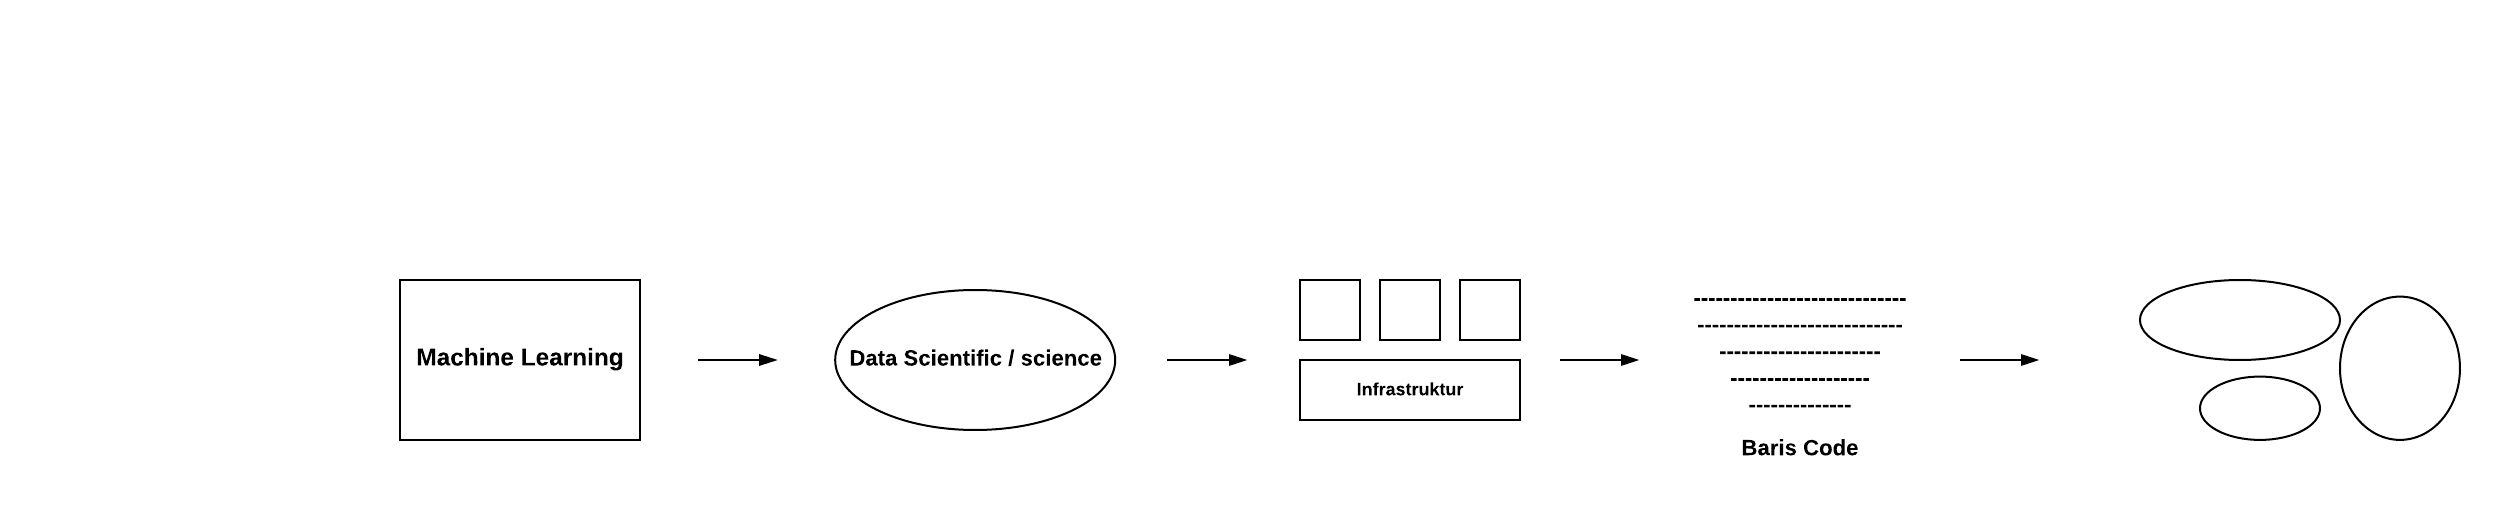
\includegraphics[width=4cm]{figures/1174054/1/3.png}
		\centering
		\caption{Module Not Found Error}
	\end{figure}
	\begin{figure}[H]
		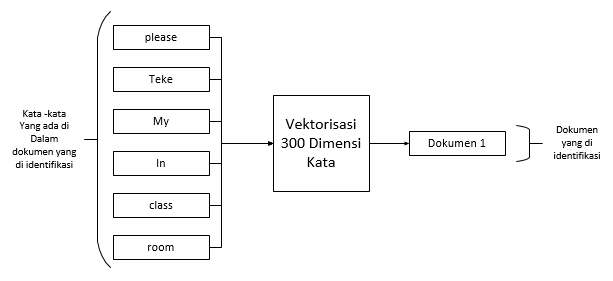
\includegraphics[width=4cm]{figures/1174054/1/4.png}
		\centering
		\caption{Import Error}
	\end{figure}

	\item Tuliskan Kode Error dan Jenis Error
	\begin{itemize}
		\item Module Not Found Error
		\item Import Error
	\end{itemize}
	\item Cara Penanganan Error
	\begin{itemize}
		\item Module Not Found Error
		\hfill\break
		Dengan memperbaiki penulisan atau kesalahan dalam penulisan kode atau melakukan install package atau modul yang belum terinstal
		\item Import Error
		\hfill\break
		Dengan Menginstall Library Yang Tidak Ditemukan
	\end{itemize}
\end{enumerate}


\subsection{Bukti Tidak Plagiat}
\begin{figure}[H]
	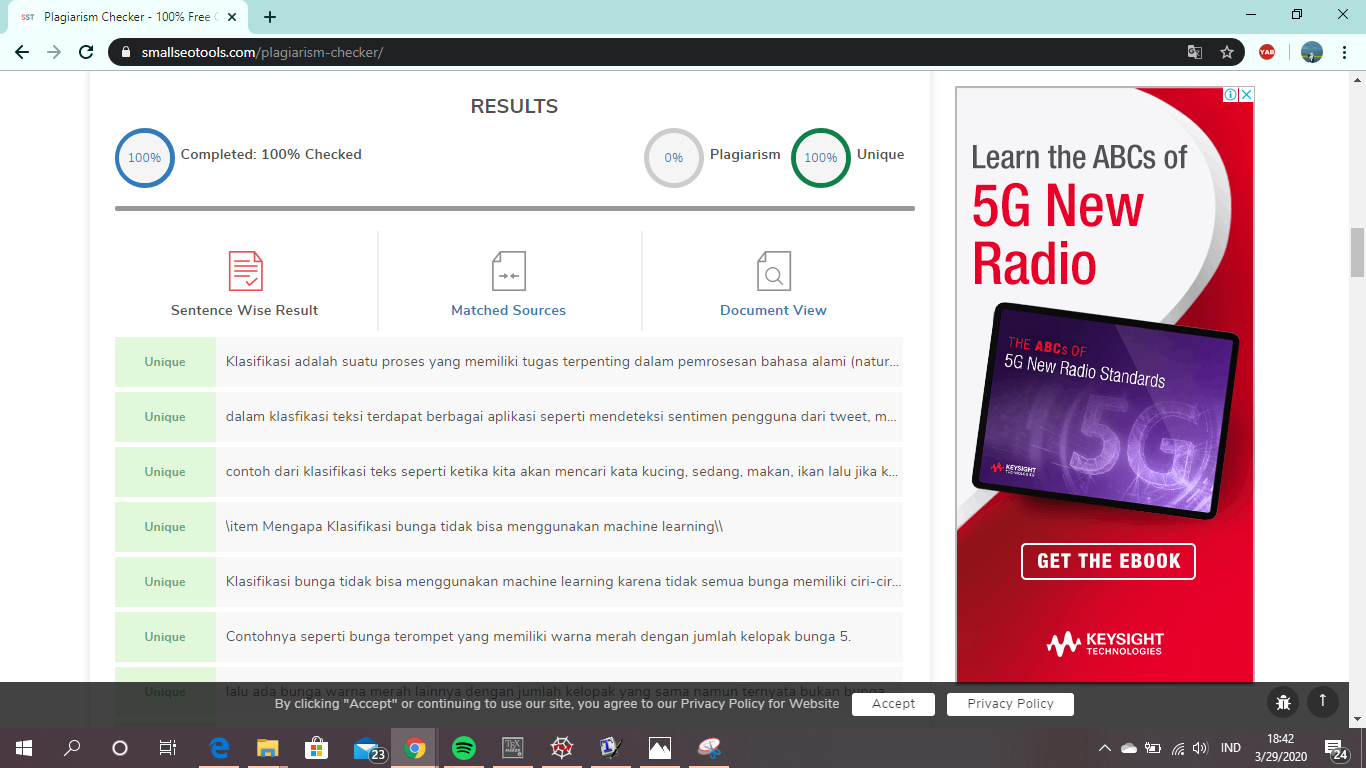
\includegraphics[width=4cm]{figures/1174054/1/plagiarisme.png}
	\centering
	\caption{Bukti Plagiasrisme}
\end{figure}

\subsection{Link Youtube}
https://youtu.be/gl9Q60DzEfI
\section{Chandra Kirana Poetra (1174079)}
\subsection{Teori}
\begin{enumerate}
\item Definisi Kecerdasan buatan\\ 
Dalam bidang komputer, Aritificial Intelligence (AI), atau biasa disebut juga sebagai Machine Intelligence merupakan bentuk dari representasi kecerdasan yang dilakukan oleh mesin, hampir mirip seperti bagaimana manusia melakukan kecerdasan. Beberapa sumber mendefinisikan  bahwa bidang yang mempelajari suatu agen kecerdasan merupakan suatu alat yang mengenali lingkungan sekitarnya dan mencoba untuk membuat kesimpulan untuk memaksimalkan kemungkinan tingkat keberhasilan dari pencapaian yang ingin dituju.

\item Sejarah dan Perkembangan Kecerdasan Buatan
\begin{itemize}
\item Pada tahun 1943, pekerjaan pertama yang dikenal sebagai AI telah dilakukan oleh Warren McCulloch dan juga Walter Pits yang dinamakan sebagai artificial neurons
\item Pada tahun 1955, Allen Newell dan Herbert A. Simon membuat program kecerdasan buatan pertama yang dinamakan Logic Theorist
\item Pada tahun 1972, robot pertama dibuat di jepang dengan nama Wabot-1 dengan kecerdasan buatan
\item Pada tahun 1980, muncul bidang baru dari kecerdasan buatan yaitu Expert System yang membantu dalam pemberian keputusan
\item Tahun 1997, IBM deep blue mengalahkan juara catur dunia Gary Kasparov dan menjadi komputer pertama yang mengalahkannya
\item Tahub 2006, perusahaaan sudah mulai menerapkan kecerdasan buatan pada produknya seperti Netflix dan Twitter.
\item Tahun 2018,  	Project Debater dari IBM melakuakn debat tentang topik yang kompleks dan berakhir dengan hasil memuaskan
\end{itemize}

\item Definisi Supervised Learning\\
Supervised Learning adalah proses untuk melatih mesin secara input dan output melalui contoh nyata secara langsung

\item Klasifikasi Supervised Learning
\begin{itemize}
\item Support Vector Machines
\item linear regression
\item logistic regression
\item naive Bayes
\item linear discriminant analysis
\item decision trees
\item k-nearest neighbor algorithm
\item Neural Networks (Multilayer perceptron)
\item Similarity learning
\end{itemize}

\item Regresi dan Unsupervised Learning\\
Regresi adalah suatu proses statistikal yang mengestimasi hubungan antara variable satu dengan variable yang lainnya.

Unsupervised Learning adalah bentuk dari machine learning yang mencari bentuk atau hubungan dari data set yang tidak mempunyai label dengan bantuan yang minimal dari manusia.

\item Dataset\\
Dataset adalah koleksi suatu data

\item Training Set\\
Training Set merupakan data yang digunakan untuk keperluan pembelajaran yang biasanya digunakan oleh machine learning

\item Testing Set\\
Testing set adalah data yang real yang digunakan untuk melatih machine learning

\end{enumerate}

\subsection{Instalasi}
\begin{enumerate}
	\item Instalasi Library scikit dari a naconda, mencoba kompilasi dan uji coba ambil contoh kode dan lihat variabel explorer
	\hfill\break
	\begin{figure}[H]
		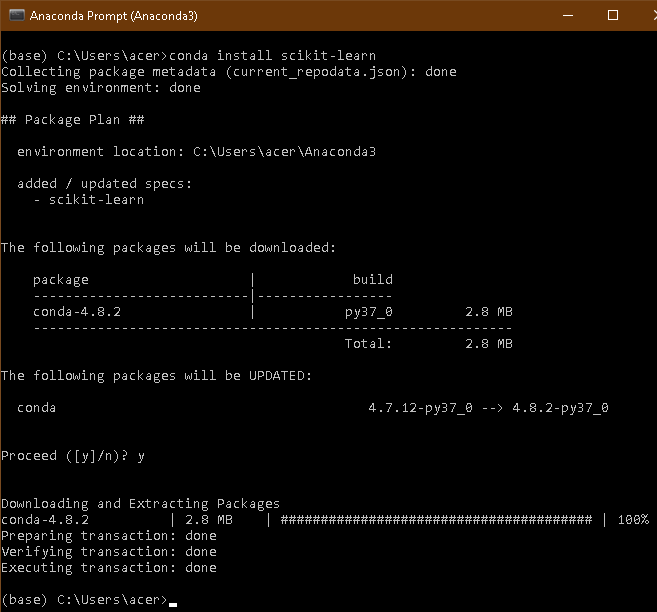
\includegraphics[width=4cm]{figures/1174079/1/1.PNG}
		\centering
		\caption{Instalasi Package Scikit Learn}
	\end{figure}
	\begin{figure}[H]
		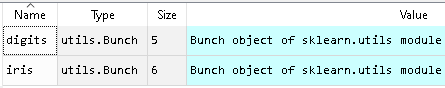
\includegraphics[width=4cm]{figures/1174079/1/2.png}
		\centering
		\caption{Isi Variabel Explorer}
	\end{figure}
	\item Mencoba Loading an example dataset, menjelaskan maksud dari tulisan tersebut dan mengartikan           		  per baris
	\hfill\break
	\lstinputlisting[firstline=2, lastline=7]{src/1174079/1/1174079.py}
	\item Mencoba Learning and predicting, menjelaskan maksud dari tulisan tersebut dan mengartikan per  			  baris
	\hfill\break
	\lstinputlisting[firstline=9, lastline=28]{src/1174079/1/1174079.py}
	\item  Mencoba Model persistence, menjelaskan maksud dari tulisan tersebut dan mengartikan per baris
	\hfill\break
	\lstinputlisting[firstline=30, lastline=48]{src/1174079/1/1174079.py}
	\item Mencoba Conventions, menjelaskan maksud dari tulisan tersebut dan mengartikan per baris
	\hfill\break
	\lstinputlisting[firstline=50, lastline=72]{src/1174079/1/1174079.py}
\end{enumerate}

\subsection{Penanganan Error}
\begin{enumerate}
	\item ScreenShoot Error
	\begin{figure}[H]
		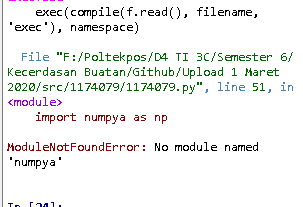
\includegraphics[width=4cm]{figures/1174079/1/error.png}
		\centering
		\caption{No Module Named Numpya}
	\end{figure}

	\item Tuliskan Kode Error dan Jenis Error
	\begin{itemize}
		\item ModuleNotFoundError
	\end{itemize}
	\item Cara Penangan Error
	\begin{itemize}
		\item ModuleNotFoundError
		\hfill\break
		Mengecek Typo dan menulis kembali library yang akan diimport
	\end{itemize}
\end{enumerate}

\subsection{Bukti Tidak Plagiat}
\begin{figure}[H]
	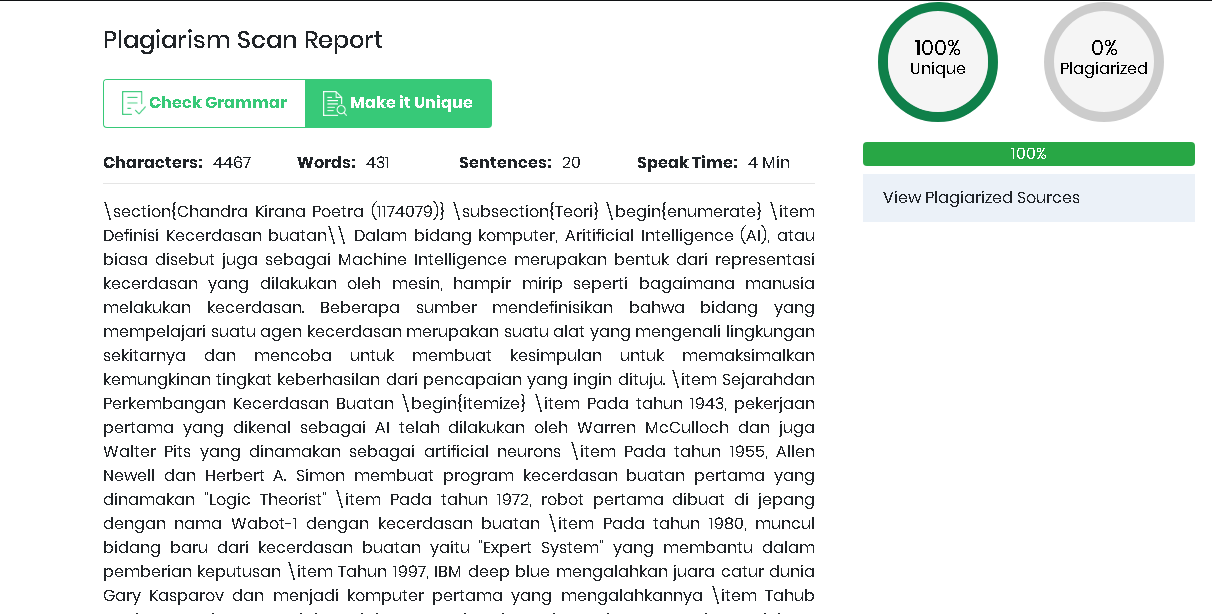
\includegraphics[width=4cm]{figures/1174079/1/plagiarism.PNG}
	\centering
	\caption{Bukti Tidak Melakukan Plagiat Chapter 1}
\end{figure}

\subsection{Link Youtube}
https://youtu.be/nPua0lRXjO8

\chapter{Chapter 2}
\input{chapters/chapter2/1174006}

\chapter{Chapter 3}
\input{chapters/chapter3/1174006}

\chapter{Chapter 4}
\input{chapters/chapter4/1174006}

\chapter{Chapter 5}
\input{chapters/chapter5/1174006}

\chapter{Chapter 6}
\input{chapters/chapter6/1174006}

\chapter{Chapter 7}
\input{chapters/chapter7/1174006}

\bibliographystyle{IEEEtran} 
%\def\bibfont{\normalsize}
\bibliography{references}


%%%%%%%%%%%%%%%
%%  The default LaTeX Index
%%  Don't need to add any commands before \begin{document}
\printindex

%%%% Making an index
%% 
%% 1. Make index entries, don't leave any spaces so that they
%% will be sorted correctly.
%% 
%% \index{term}
%% \index{term!subterm}
%% \index{term!subterm!subsubterm}
%% 
%% 2. Run LaTeX several times to produce <filename>.idx
%% 
%% 3. On command line, type  makeindx <filename> which
%% will produce <filename>.ind 
%% 
%% 4. Type \printindex to make the index appear in your book.
%% 
%% 5. If you would like to edit <filename>.ind 
%% you may do so. See docs.pdf for more information.
%% 
%%%%%%%%%%%%%%%%%%%%%%%%%%%%%%

%%%%%%%%%%%%%% Making Multiple Indices %%%%%%%%%%%%%%%%
%% 1. 
%% \usepackage{multind}
%% \makeindex{book}
%% \makeindex{authors}
%% \begin{document}
%% 
%% 2.
%% % add index terms to your book, ie,
%% \index{book}{A term to go to the topic index}
%% \index{authors}{Put this author in the author index}
%% 
%% \index{book}{Cows}
%% \index{book}{Cows!Jersey}
%% \index{book}{Cows!Jersey!Brown}
%% 
%% \index{author}{Douglas Adams}
%% \index{author}{Boethius}
%% \index{author}{Mark Twain}
%% 
%% 3. On command line type 
%% makeindex topic 
%% makeindex authors
%% 
%% 4.
%% this is a Wiley command to make the indices print:
%% \multiprintindex{book}{Topic index}
%% \multiprintindex{authors}{Author index}

\end{document}

